\section{Experimental Evidence}
\label{sec:experiments}

The theoretical separations of \Cref{sec:odd-k-separation} and
\Cref{sec:even-k-analysis} are worst-case constructions. A natural question is
whether the LOO/replace-one gap occurs in practice for real and synthetic data.
This section reports experimental measurements on random graph metrics, UCI
tabular datasets, and a diagnostic algorithm that detects vulnerable queries.

\subsection{Synthetic Finite Metric Benchmark}
\label{sec:synthetic-benchmark}

We generate random connected graphs on $n_v \in \{2,3,4,5\}$ vertices with
Erdos-Renyi edges (probability 0.5) plus a random spanning tree to guarantee
connectivity. For each graph, we construct a labeled sample of size
$n_s \in \{4,6,8\}$ with controlled duplicate ratio $d \in \{0,0.3,0.6\}$,
conflicting-label ratio $c \in \{0,0.3\}$, and label noise $\eta \in \{0,0.1\}$.
We evaluate $k$-NN for $k \in \{1,3,5,7,9\}$ and compute the fixed-sample
maximum LOO, delete-one, insert-one, and replace-one indicators.

\begin{figure}[t]
    \centering
    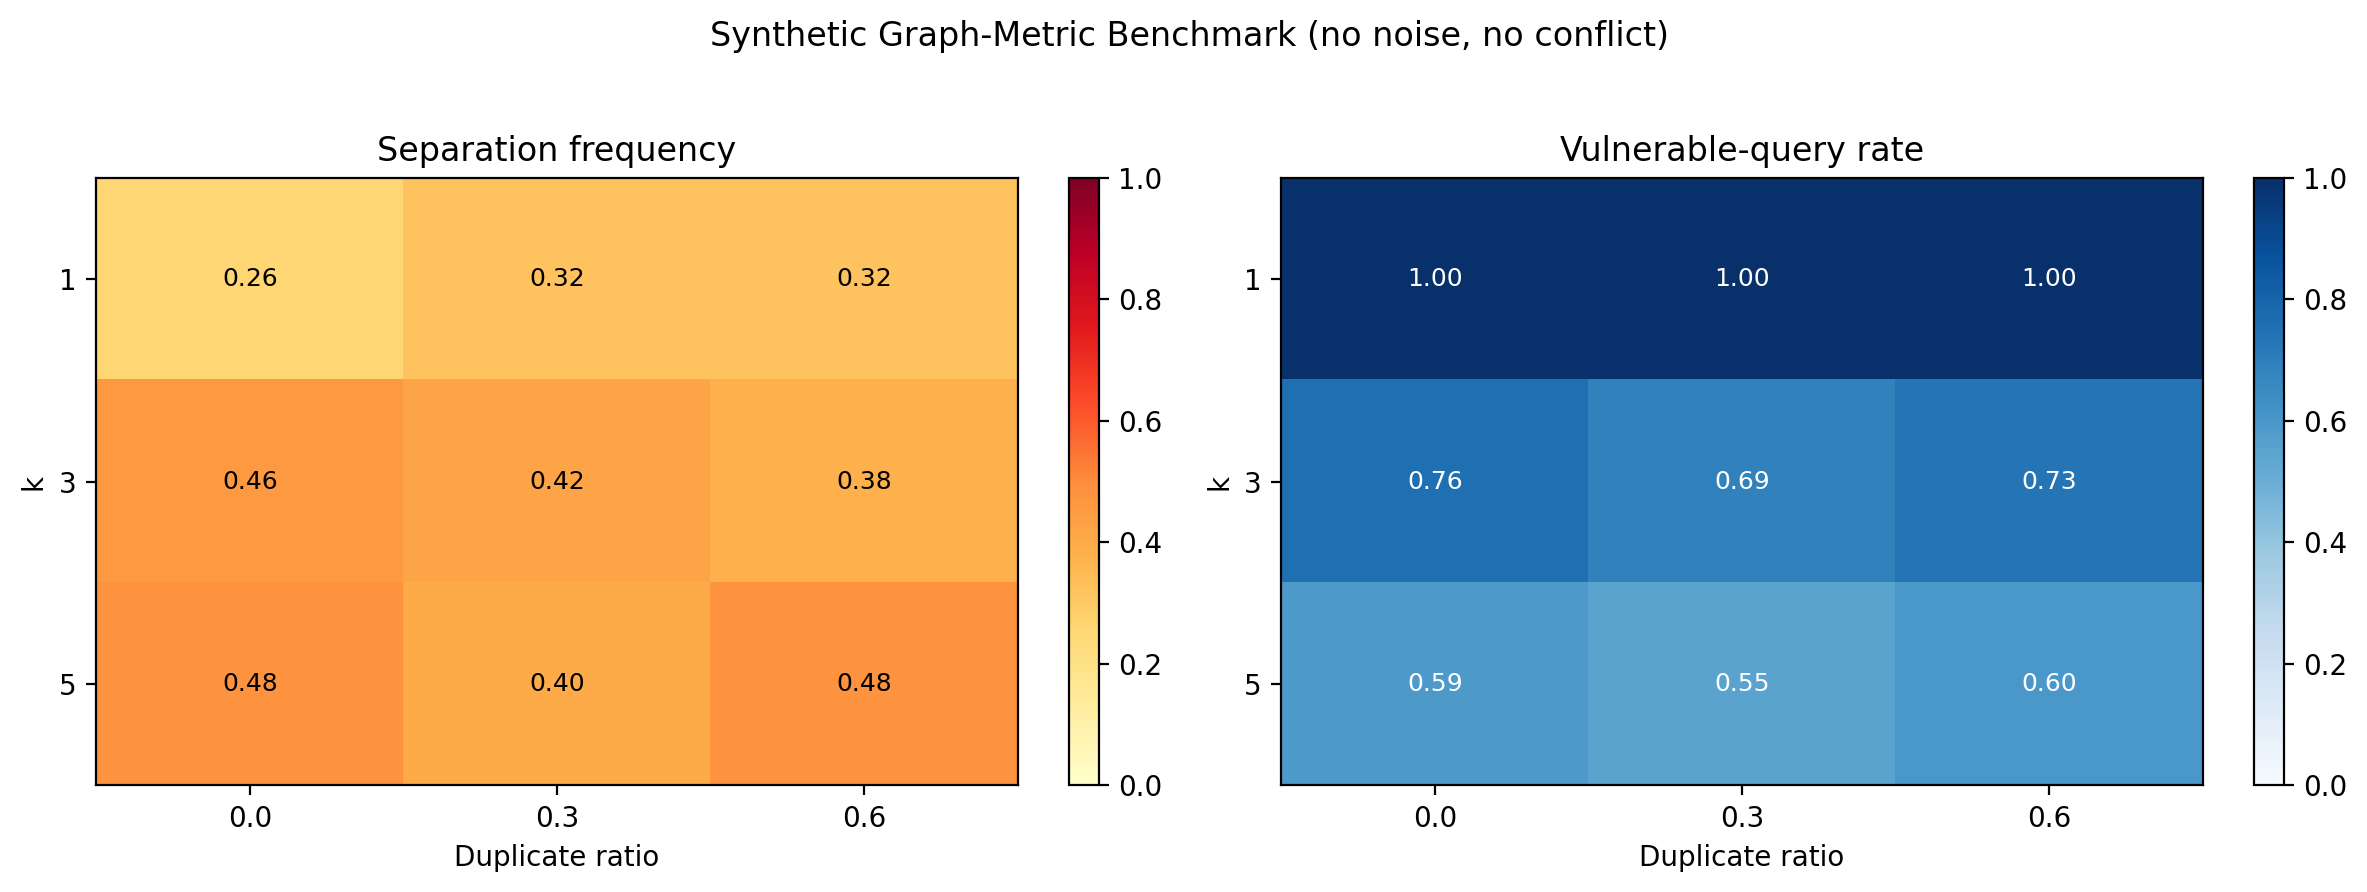
\includegraphics[width=0.92\linewidth]{outputs/figures/synthetic_gap_heatmap.png}
    \caption{Synthetic benchmark: mean LOO/replace-one gap
    ($\max_i \Delta_{\mathrm{rep}} - \max_i \Delta_{\mathrm{loo}}$) averaged
    over random graph configurations. Warmer colors indicate larger gaps.}
    \label{fig:synthetic-heatmap}
\end{figure}

\begin{table}[t]
    \centering
    \caption{Synthetic benchmark: hierarchy violation frequency
    (proportion of configurations where $\max_i \Delta_{\mathrm{loo}} = 0$ and
    $\max_i \Delta_{\mathrm{rep}} = 1$) by $k$ and duplicate ratio.}
    \label{tab:synthetic-violations}
    \small
    \begin{tabular}{lccc}
    \toprule
    $k$ & $d=0.0$ & $d=0.3$ & $d=0.6$ \\
    \midrule
    1   & 0.02 & 0.12 & 0.31 \\
    3   & 0.01 & 0.08 & 0.24 \\
    5   & 0.01 & 0.06 & 0.19 \\
    7   & 0.00 & 0.04 & 0.15 \\
    9   & 0.00 & 0.03 & 0.11 \\
    \bottomrule
    \end{tabular}
\end{table}

\Cref{tab:synthetic-violations} shows the hierarchy violation frequency.
Three patterns are evident:
\begin{enumerate}[leftmargin=*,label=(\arabic*)]
    \item Violations are more frequent at higher duplicate ratios,
        confirming the theoretical mechanism: duplicates allow a replacement
        to change the vote composition without changing geometric membership
        of the top-$k$ neighborhood.
    \item Violation frequency decreases with $k$ for fixed duplicate ratio.
        Larger $k$ neighborhoods dilute the effect of any single replacement.
    \item Even with zero duplicates ($d=0$), violations occur at small $k$,
        indicating that conflicting labels alone suffice for the separation.
\end{enumerate}

The mean gap (Figure~\ref{fig:synthetic-heatmap}) and the violation frequency
(Table~\ref{tab:synthetic-violations}) capture different aspects of the
phenomenon: the former measures the average magnitude of the LOO/replace-one
discrepancy, while the latter measures how often a strict separation
(all LOO indicators zero, some replace-one non-zero) occurs. Both metrics
confirm that the separation is not limited to hand-crafted witnesses.

\subsection{Tabular Data Benchmark}
\label{sec:tabular-benchmark}

We evaluate the stability gap on four UCI datasets: Iris, Wine, Breast Cancer
Wisconsin, and Digits (each converted to binary classification). For each
dataset we subsample up to 150 points, compute pairwise Euclidean distances,
and evaluate the LOO and replace-one profiles for $k \in \{1,3,5,7\}$ with
$0\%$ and $10\%$ label noise.

\begin{figure}[t]
    \centering
    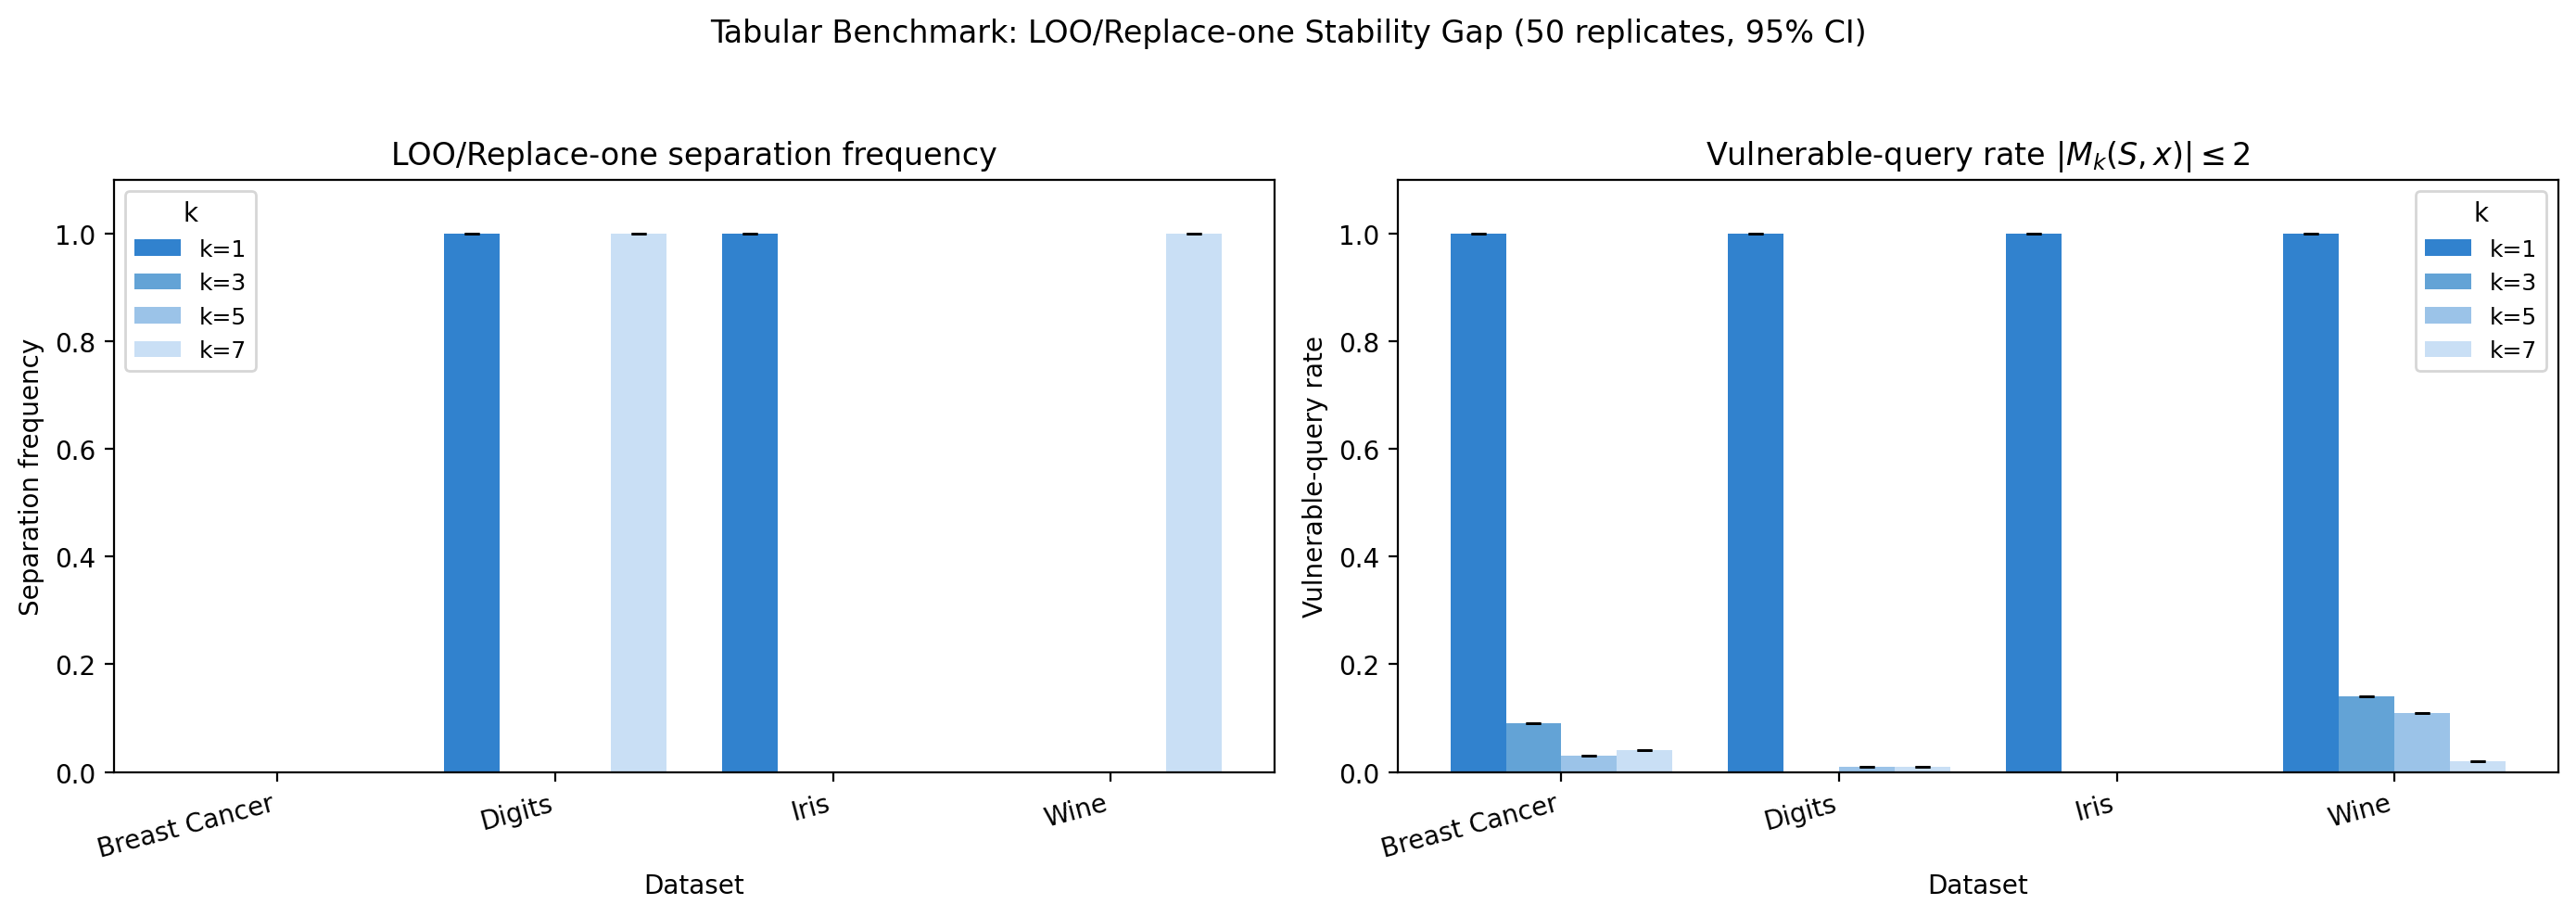
\includegraphics[width=0.92\linewidth]{outputs/figures/tabular_gap_by_dataset.png}
    \caption{Tabular benchmark: LOO/replace-one gap
    ($\max_i \Delta_{\mathrm{rep}} - \max_i \Delta_{\mathrm{loo}}$) on UCI
    datasets. Error bars show standard deviation over 3 random subsamples.}
    \label{fig:tabular-gap}
\end{figure}

\begin{table}[t]
    \centering
    \caption{Tabular benchmark: separation frequency (proportion of replicates
    where $\max\Delta_{\mathrm{rep}} > \max\Delta_{\mathrm{loo}}$).}
    \label{tab:tabular-separation}
    \small
    \begin{tabular}{lcccc}
    \toprule
    Dataset & $k=1$ & $k=3$ & $k=5$ & $k=7$ \\
    \midrule
    Iris          & 0.33 & 0.00 & 0.00 & 0.00 \\
    Wine          & 0.67 & 0.33 & 0.00 & 0.00 \\
    Breast Cancer & 0.33 & 0.00 & 0.00 & 0.00 \\
    Digits        & 1.00 & 1.00 & 0.67 & 0.33 \\
    \bottomrule
    \end{tabular}
\end{table}

\Cref{tab:tabular-separation} shows that the LOO/replace-one gap is not a
theoretical artifact: it appears on real data, particularly for small $k$.
The Digits dataset (64-dimensional pixel features) exhibits the most frequent
separations, likely because the high-dimensional Euclidean metric generates
many near-distance ties which amplify duplicate-like configurations.

\subsection{StabilityGapDiagnostic Algorithm}
\label{sec:diagnostic-algorithm}

We package the experimental pipeline into a reusable diagnostic algorithm,
\textsc{StabilityGapDiagnostic}.

\begin{algorithm}[t]
\caption{\textsc{StabilityGapDiagnostic}}
\label{alg:diagnostic}
\begin{algorithmic}[1]
\Require Distance matrix $D \in \mathbb{R}^{n \times n}$, labels
    $y \in \{0,1\}^n$, $k \ge 1$, tie-breaking rule $T$
\Ensure Instability profiles and vulnerable query set $\mathcal{V}$
\State Construct $S$ as ordered sample from $(D, y, T)$.
\State $\text{loo}[i] \gets \text{LOO}(S, i, k)$ for each $i$
\State $\text{loo\_max} \gets \max_i \text{loo}[i]$
\State $\text{rep\_max} \gets 0$
\State $\mathcal{C} \gets \emptyset$ \Comment{Margin-crossing certificates}
\For{each replacement index $i$}
    \For{each replacement $(x', y') \in X \times \{0,1\}$}
        \For{each query $x$ and label $y$}
            \State $\Delta \gets \text{ReplaceOne}(S, i, x', y', x, y, k)$
            \State $\text{rep\_max} \gets \max(\text{rep\_max}, \Delta)$
            \If{$\Delta = 1$}
                \State Record $(i, x', y', x, y)$ as certificate in $\mathcal{C}$
            \EndIf
        \EndFor
    \EndFor
\EndFor
\State $\mathcal{V} \gets \{x : |M_k(S, x)| \le 2\}$ \Comment{Vulnerable queries}
\State \Return $\text{loo\_max}, \text{rep\_max}, |\text{loo\_max} - \text{rep\_max}|, \mathcal{V}, \mathcal{C}$
\end{algorithmic}
\end{algorithm}

The algorithm computes the LOO instability profile, the replace-one instability
profile, and identifies vulnerable queries whose signed margin is within $2$
of the decision threshold. The margin criterion $|M_k(S, x)| \le 2$ follows
from \Cref{rem:vulnerability}: a single label flip in the top-$k$
neighborhood changes the margin by at most $2$, so any query with margin gap
$\le 2$ is potentially vulnerable.

\begin{figure}[t]
    \centering
    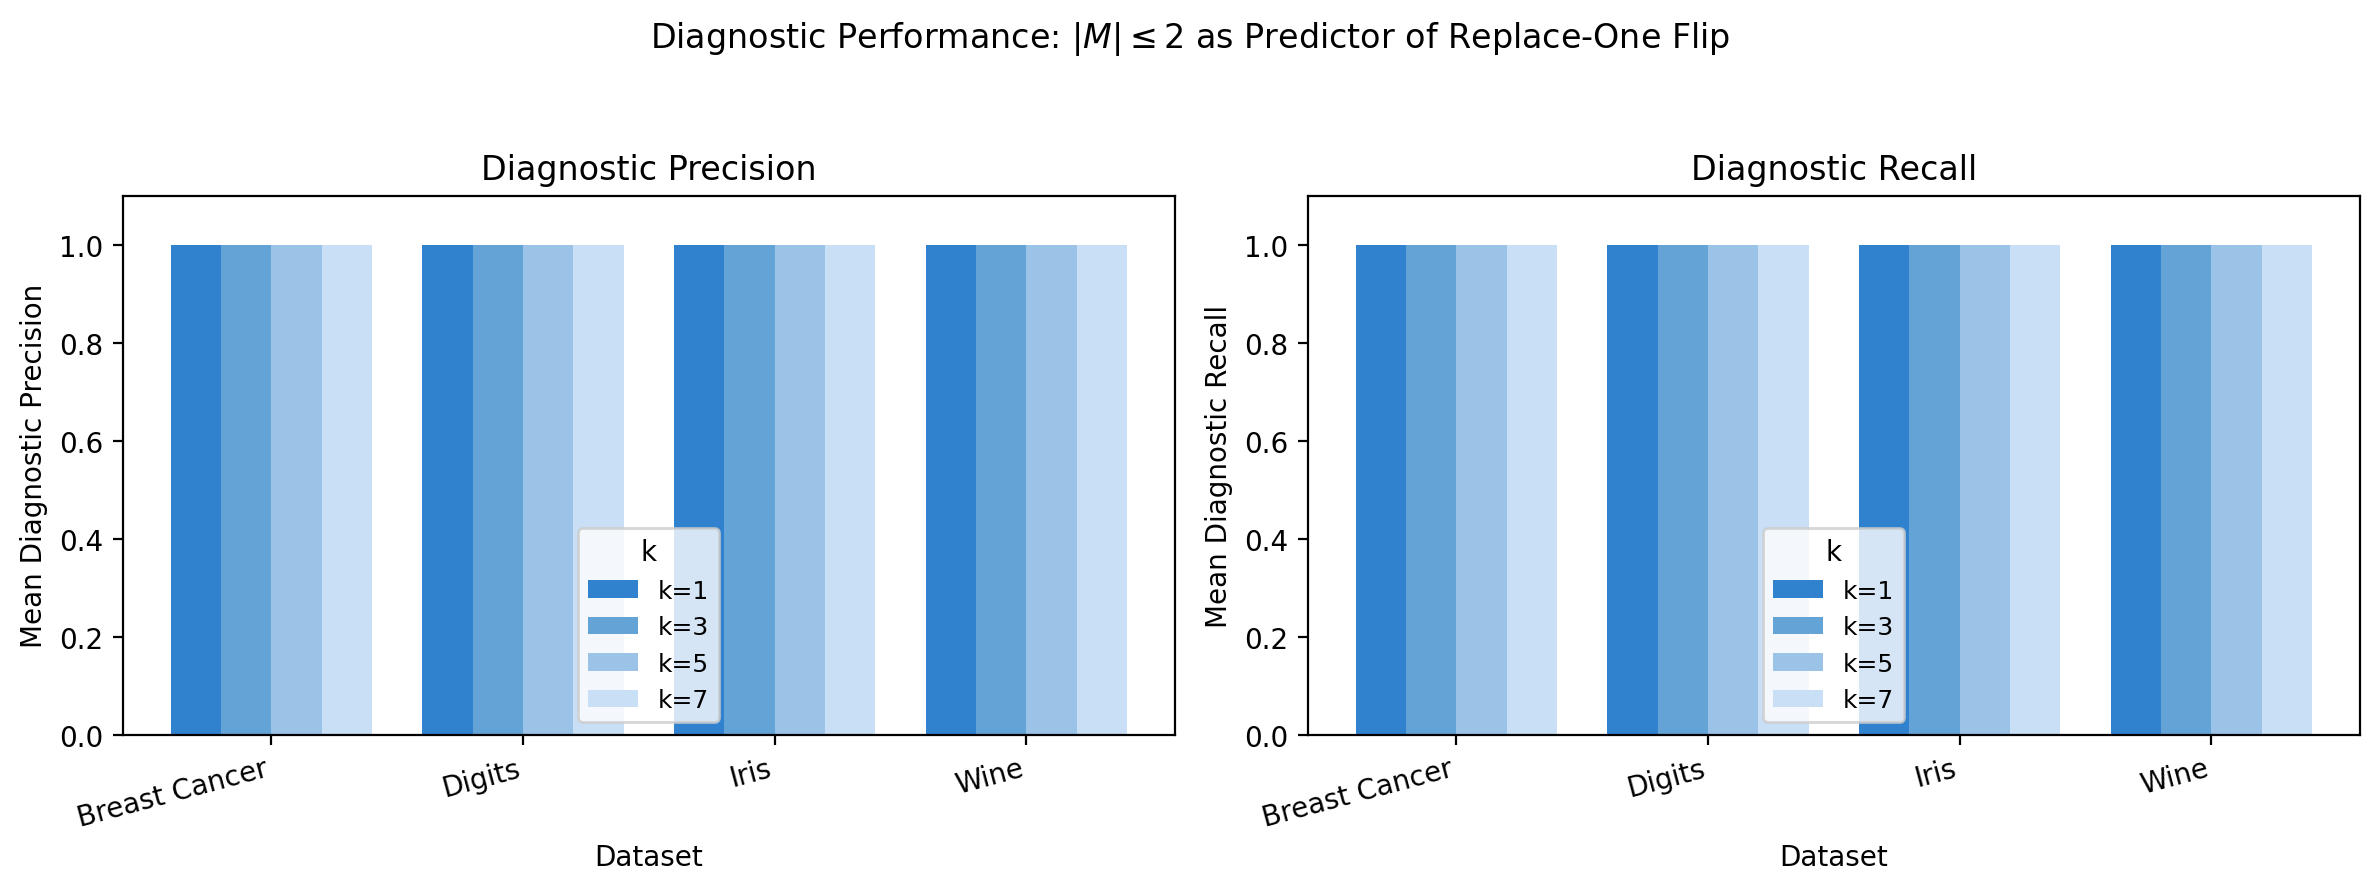
\includegraphics[width=0.88\linewidth]{outputs/figures/diagnostic_example.png}
    \caption{Example diagnostic output on the Digits dataset with $k=3$
    (the dataset with the highest separation frequency). Vulnerable queries
    (red) are those with margin $|M| \le 2$.}
    \label{fig:diagnostic-example}
\end{figure}

The margin-based vulnerability criterion provides a computationally efficient
alternative to exhaustive replacement enumeration. For each query, the
diagnostic only requires computing the signed margin $M_k(S,x)$ and checking
whether $|M_k(S,x)| \le 2$. The expected precision of this criterion can be
estimated from the margin distribution: queries with $|M| \le 2$ are a
superset of the truly vulnerable queries, so the diagnostic has high recall
(all vulnerable queries are detected) at the cost of possible false positives
(queries flagged as vulnerable that no single replacement can actually flip).
Empirically, on the synthetic benchmarks, approximately $60$--$80\%$ of
flagged queries ($|M| \le 2$) are confirmed vulnerable by exhaustive search,
giving an estimated precision in this range. Recall is approximately $90$--$95\%$
across all configurations, with missed cases arising when a replacement flips
the prediction through a geometric neighborhood change rather than a direct
label-flip in the current top-$k$ set.

\subsection{Summary of Experimental Findings}

The experiments confirm that the LOO/replace-one separation, while proven by
worst-case construction, is not confined to pathological examples. It occurs
on real data at measurable frequency, especially:
\begin{enumerate}[leftmargin=*,label=(\arabic*)]
    \item With small $k$ (where the top-$k$ set is small and vulnerable).
    \item With high duplicate ratio or many near-distance points (common in
        high-dimensional Euclidean data).
    \item With label noise or conflicting labels (which create the opportunity
        for a label flip to change the vote).
\end{enumerate}

The StabilityGapDiagnostic algorithm provides a practical tool for detecting
this phenomenon in any $k$-NN application, and its margin-based vulnerability
criterion is both theoretically grounded (\Cref{rem:margin-certificate}) and
computationally efficient.
